%----------------------------------------------------------------------------------------
%	PACKAGES AND DOCUMENT CONFIGURATIONS
%----------------------------------------------------------------------------------------
\documentclass[11pt]{article}
\usepackage{amsmath} % Required for some math elements
\usepackage{hyperref} 
\usepackage{xcolor}
\usepackage{lipsum} 
\usepackage{cite}
\usepackage{graphicx} % Required for the inclusion of images
\usepackage{algorithmic}
\usepackage{array}
\usepackage{bookmark}
\usepackage{listings}
\usepackage{amssymb}
\usepackage{enumitem}   
\usepackage[margin=16mm]{geometry}
\usepackage[caption=false, font=footnotesize]{subfig}

\newlist{steps}{enumerate}{1}
\setlist[steps, 1]{label = Step \arabic*:}

\hypersetup{ %color attributes of citation, link, etc.
    colorlinks=true,
    linkcolor=blue,
    filecolor=gray,      
    urlcolor=blue,
    citecolor=blue,
}

\newcommand{\matlab}{\textsc{Matlab}} %very important and totally necessary addition

\newcommand\Item[1][]{%
  \ifx\relax#1\relax  \item \else \item[#1] \fi
  \abovedisplayskip=0pt\abovedisplayshortskip=0pt~\vspace*{-\baselineskip}}
%----------------------------------------------------------------------------------------
%	DOCUMENT INFORMATION
%----------------------------------------------------------------------------------------
 
\title{ECEN321: Analogue Electronics \\ Assignment 1: Power Amplifiers - Submission}
\author{Daniel Eisen : 300447549}
\date{\today}

\begin{document}
\maketitle
%----------------------------------------------------------------------------------------
%	DOCUMENT CONTENT
%----------------------------------------------------------------------------------------
\section*{Question 1}
  \begin{enumerate}[label = \Roman*.]
          \item \textit{An audio amplifier operates in the frequency range of..} \\ 
          \textbf{a. 20Hz to 20kHz} 

          \item \textit{For maximum peak-to-peak output voltage, the Q point should be..} \\ 
          \textbf{c. At the centre of the dc load line}
          
          \item \textit{An amplifier has two load lines because..} \\ 
          \textbf{d. All of the above} 
          
          \item \textit{Push-pull is almost always used with..} \\ 
          \textbf{b. Class B} 
          
          \item \textit{Class C amplifiers are almost always..} \\ 
          \textbf{c. Tuned RF amplifiers} 
          
          \item \textit{The input signal of a class C amplifier..} \\ 
          \textbf{c. Produces brief pulses of collector current} 
          
          \item \textit{If RC=100Ω and RL=180Ω, the ac load resistance equals..} \\ 
          \textbf{a. 64Ω} 
          
          \item \textit{In a class A amplifier, the collector current flows for..} \\ 
          \textbf{d. The entire cycle} 
          
          \item \textit{With class A, the output signal should be..} \\ 
          \textbf{a. Unclipped} 
          
          \item \textit{A small quiescent current is necessary with a class AB push-pull amplifier to avoid..} \\ 
          \textbf{a. Crossover distortion} 
  \end{enumerate}

  \newpage
  \section*{Question 2}
  \begin{enumerate}[label=\alph*)]
    \item % a)
    In the push push-pull configuration, the base-emitter junctions of the transistors have a potential of 0.7V. Thus when the input drops below this, at the \textbf{crossover} around the zero-point, the output is cut-off. This introduces a flatline distortion between positive and negative half cycles.
    
    \item % b)
   
    \begin{figure}[h]
      \centering
      \subfloat[Voltage-Divider Bias]{%
              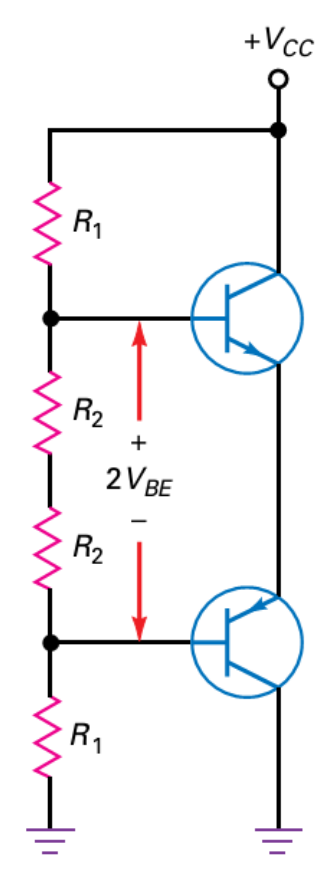
\includegraphics[width=0.15\linewidth]{inc/push_pull_R.png}}
              \hspace{0.15\linewidth}
      \subfloat[Diode Bias]{
              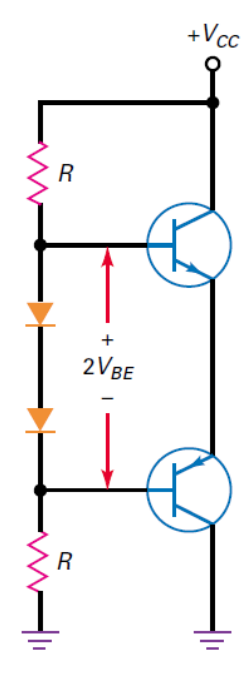
\includegraphics[width=0.15\linewidth]{inc/push_pull_D.png}}
      \caption{Class B/AB Biasing Configurations}
      \label{fig_graph} 
    \end{figure} 

    Figure 1a shows a voltage-divider biasing configuration with a summed potential difference of $2V_{BE}$ to unsure the transistors are always on, so the avoid the crossover distortion. The issue with this being high temperature sensitivity with the ultimate issue being thermal runaway. 

    Figure 1b shows a diode biasing configuration, this is a way to avoid thermal runaway and still providing the same potential difference. The curves of the compensating diodes must match the $V_{BE}$ curves of the transistors so temperature changes result in an adjusted bias voltage.


  \end{enumerate}
  
\newpage
\section*{Question 3}
  $V_{CC} = +20V \; R_{1,2} = 1k \; R_C = 50\Omega \; R_E = 100\Omega \; R_L = 50\Omega$

  \begin{enumerate}[label=\roman*)]
    \Item % input power
      \begin{align*}
        P_{i(dc)} &= V_{CC}{\cdot}I_{CQ} \\
        V_{B} &= \frac{R_{2}}{R_{1}+R_{2}}V_{CC} = \frac{1k}{1k+1k}20V = 10V \\
        V_{E} &= V_{B} - 0.7 = 9.3V \\
        I_{E} &= \frac{V_{E}}{R_{E}} = \frac{9.3}{100} = 93mA \approx I_{CQ} \\
        \therefore P_{i(dc)} &= 20 \times 93mA = 1.86W \\
      \end{align*}

    \Item % output power
      \begin{align*}
        P_{o(ac)} &= \frac{V_{CEQ}{\cdot}I_{CQ}}{2} \\
        V_{CEQ}   &= V_{C} - V_{E} = (V_{CC} - I_{C}{\cdot}R_{C}) - V_{E} \\
                  &= (20V - 93mA \times 50\Omega) - 9.3V = 6.05V \\ 
        \therefore P_{o(ac)} &= \frac{6.05V \times 93mA}{2} = 0.28W \\
      \end{align*}

    \Item % efficiency.
      \begin{align*}
        \% \eta &= \frac{P_{o(ac)}}{P_{i(dc)}} \times 100 \\
                &= \frac{0.28}{1.86} \times 100 = 15\%  \\
      \end{align*}
  \end{enumerate}


\section*{Question 4}
  $V_{CC}=V_{CEQ}=5V \;\; I_{CQ}=50mA$

  \begin{enumerate}[label=\roman*)]
    \Item % maximum  a.c. power output
      \begin{align*}
        P_{o(ac \; max)} &= \frac{I_{CQ}{\cdot}V_{CEQ}}{2} \\
        &= \frac{50mA{\times}5V}{2} = 0.125W \\
      \end{align*}
    \Item % power rating of transistor (DC input power for this application)
      \begin{align*}
        P_{i(dc)} &= I_{CQ}{\cdot}V_{CEQ} \\
        &= 50mA{\times}5V = 0.25W \\
      \end{align*}
    \Item % maximum efficiency.
      \begin{align*}
        \% \eta_{max} &=  \frac{P_{o(ac \; max)}}{P_{i(dc)}} \times 100 \\
        &= \frac{\frac{I_{CQ}{\cdot}V_{CEQ}}{2}}{I_{CQ}{\cdot}V_{CEQ}} \times 100 \\
        &= \frac{0.125}{0.25} \times 100 = 50\% \\
      \end{align*}
  \end{enumerate}
  
  \newpage
\section*{Question 5}
  $V_{CC} = +30V \; V_{BE} = 0.7V \; R_{1} = 300\Omega \; R_L = 16\Omega$\
  
  \begin{align*}
    V_{CC} &= 2R_{1}{\cdot}I + 2V_{BE} \\
    30V &= 600\Omega \times I + 1.4V \\
    I &= \frac{30V-1.4V}{600\Omega} = 47.67mA \\
    R_{2} &= \frac{V_{BE}}{I} = \frac{0.7V}{47.67mA} = 14.67\Omega  \\
  \end{align*}

\section*{Question 6}
$f=3\mathrm{MHz} \; V_{CC} = 20V \; V_{CE(sat)} = 0.3V \; I_{P}=500mA$
\begin{enumerate}[label=\roman*)]
  \Item % Efficiency
    \begin{align*}
      V_{P} &= V_{CC} - V_{CE(sat)} \\
      &= 20V - 0.3 = 19.7V \\
      P_{)} &= \frac{V_{P}^{2}}{2R_{L}} = \frac{388.09}{200} = 1.94W \\
      I_{dc} &= \frac{P_{O}}{V_{P}} = \frac{1.94}{19.7} = 98.5mA \\
      P_{dc} &= V_{CC}{\cdot}I_{dc} = 20 \times 98.5 = 1.97W \\
      \% \eta &= \frac{P_{O}}{P_{dc}} \times 100 = \frac{1.94}{1.97} \times 100 \\ &= 98.5\% \\ 
    \end{align*}
  \Item % Conduction Angle
    \begin{align*}
      T &= \frac{1}{f} = \frac{1}{3{\times}10^{6}} = 3.33{\times}10^{-7} \\
      t &= \frac{P_{O}{\cdot}T}{I_{P}{\cdot}V_{P}} = \frac{1.94{\times}3.33 {\times}10^{-7}}{500{\times}19.7} = 6.56{\times}10^{-8} \\
      \phi &= \frac{P_{O}}{P_{dc}} \times 360 = \frac{6.56{\times}10^{-8}}{3.33{\times}10^{-7}} \times 360 \\ &= 70.92^{\circ}
    \end{align*}
\end{enumerate}

\end{document}